\section{Design and Implementation}
\label{sec:design}

\begin{figure}[t] 
  \centering 
  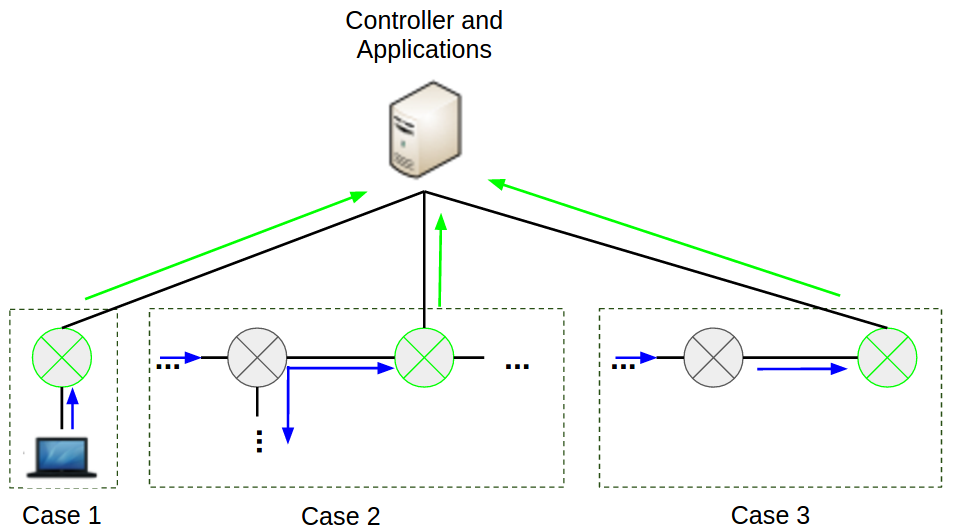
\includegraphics[width=3.3in]{img/cases.png}
  \caption{Three cases of packet\_in messages being generated at a
  switch} 
  \label{fig:cases}
\end{figure}

This section introduces \name, our proposed detection mechanism for 
network reconnaissance using packet\_in abuse. First we discuss the 
high level design decisions for both \name and the design of a 
packet\_in abuse reconnaissance attack. The design will address the
challenges listed at the end of Section~\ref{sec:overview} and 
briefly discuss the challenges and justify our implementation of a 
packet\_in abuse reconnaissance attack. Further discussion about
the trade-offs and their limitations will be covered in
Section~\ref{sec:disc}.

\subsection{Design}

Before getting into the low implementation details of \name and
the reconnaissance attack, we first examine the design of the pieces 
needed to properly implement \name and perform a packet\_in abuse 
network reconnaissance attack.

\myparagraph{\name} As described in Section~\ref{sec:overview} the key
characteristic used to identify illegitimate packet\_in messages is the
mapping between the source IP and the physical switch the packet was 
received on. Also recall packet\_in messages are generated by switches
when an incoming packet does not match any flow installed in its flow
table. This results in three cases in which a packet\_in message can be
generated at a switch. Each of these three cases  must be handled 
differently in order to detect an illegitimate packet\_in message. In 
Case 1, a host directly connected to a switch sends a packet not matching
any flows in the switch's flow table and generates a packet\_in message.
This is the simplest case as a source IP can be directly mapped to a
physical host attached to a switch's physical port. 

Packets received from other switches make validation more complex. When
a packet not matching any flows is received on a port connected to 
another switch, it is necessary to examine the previous switch to see 
how the packet was forwarded. The are two ways the previous switch may 
have forwarded the packet as described by Cases 2 and 3. In Case 2, the 
previous switch is instructed by the controller to flood a packet on 
all ports other than the port it was received on. Case 3 covers the
situation where the previous switch forwards a packet based on a match
in its flow table. 

Figure~\ref{fig:cases} visualizes each of these three cases using blue 
arrows to represent the flow of a packet and green arrows to represent 
the generation of a packet\_in message from a switch (also colored in
green) after receiving a packet that does not match any flows in its 
flow table.

In each case a packet\_in message must be validated differently. Case 1
is trivial because it simply checks if the source IP matches the
expected IP address of the host connected at that switch's physical 
port. Cases 2 and 3 do not have the luxury of easily tracing a packet to
its origin. Instead of tracing a packet all the way back to its source
hop by hop, the information at the previous switch may be used to 
validate an incoming packet. Validation of a packet\_in message in Case 
2 can be done with knowledge of packet\_in messages generated by the 
previous switch. If an application used the controller's NBI to instruct
a switch to flood a packet, then the packet\_in messages at the next hop
are considered legitimate. Similarly in Case 3, if the previous switch 
forwarded a packet using a rule from its flow table, then the presence 
of a flow installed on the switch can validate a packet\_in message on 
the next hop.

Tracking the information needed to validate packet\_in messages, such as
topology information and a log of previous flow\_mod messages, can
already be tracked using existing applications; however \name tracks
this information without the need for a trusted third party application.
This requires additional programming effort and computational overhead, 
but keeps the Trusted Computing Base minimalistic. To prevent high 
overheads on network latency and throughput, \name processes each 
packet\_in event in parallel with other applications. This allows other
applications to quickly send control messages to the controller to
install flows on a switch while \name is validating the packet\_in
message. 

\name opts to detect network reconnaissance and raise alarms rather than
preventing the attacks. This decision is two fold, first the cost of 
prevention is too high when considering false positives. False positives 
are discussed in more detail in Section~\ref{sec:disc}, but an approach
that isolates or reboots switches after an alarm is raised may cause 
severe service disruption to the network. Secondly, the damage done by 
network reconnaissance alone is not severe enough to justify taking 
preventative measures, recall network reconnaissance is an attack
phase happening just before data exfiltration, so raising an alarm for
manual analysis is an appropriate action. 

\myparagraph{Reconnaissance Attack} To ensure full coverage of the
detection capabilities of \name, the attack is constructed to spoof
packets and their physical switch port to seem like the packets are
coming from physical hosts connected to a switch and other switches. We
simulate a reconnaissance attack using packet\_in abuse by implementing
a malicious app in the application plane to edit the event port of 
packet\_in messages from certain IP ranges before they are processed by
other applications and \name. As discussed in the implementation, it is 
ensured the malicious app does not give any advantage to \name in
detecting attacks compared to attacks launched from a compromised switch.
